%------------------------------------------------------------------------------------
%	CHAPTER 5
%------------------------------------------------------------------------------------
\chapterimage{headConceito.png}
\chapter{Modelos Preditivos}

\begin{remark}
O que sabemos é uma gota; o que ignoramos é um oceano. (Isaac Newton - Astrônomo) 
\end{remark}

\section{Naïve Bayes}\index{Modelos Preditivos}
As pessoas pensam que o Cientista de Dados possui Contatos do Além e podem prever números da MegaSena ou um Desastre de Avião quando se fala em "Predição", sinto não somos charlatões, podemos pegar todos resultados da MegaSena e demonstrar com base em modelos quais os números que mais ou menos saíram, ou analisar os dados físicos de um avião, cruzar isso com todos os voos que já se acidentaram e tentar traçar uma característica. Em ambos os casos não espere certeza, existe o que chamamos: "Probabilidade de Acontecer".

Naïve Bayes é o tipo de algorítimo que dá medo em muito Cientista novato, talvez seja porque aparenta ser o mais matemático possível, sua descrição precisa seria "classificador probabilístico baseado no Teorema de Bayes, o qual foi criado por Thomas Bayes (1701 - 1761)". Para não assustar ninguém, devemos saber que trata-se de um Algorítimo Supervisionado destinado a probabilidades. Resumidamente: Qual a probabilidade de um evento A ocorrer dado que um evento B ocorreu? Qual a probabilidade de um e-mail ser spam dado que chegou um e-mail? Ativamos nosso JupyterLab personalizado que criamos com o Docker e na primeira célula importamos as bibliotecas necessárias:
\begin{lstlisting}[]
import numpy as np
import pandas as pd

from sklearn.naive_bayes import MultinomialNB
from sklearn.naive_bayes import BernoulliNB
from sklearn.naive_bayes import GaussianNB
from sklearn.model_selection import train_test_split
from sklearn.metrics import accuracy_score
\end{lstlisting}

Além das bibliotecas tradicionais como Pandas e NumPy para manipulação dos dados, temos todo o pacote da Naive\_Bayes para os três tipos do modelo:
\begin{itemize}[nolistsep]
	\item Multinominal - realizar predições quando as variáveis (categóricas ou contínuas) descrevem contas discretas de frequência.
	\item Bernoulli - realizar predições para variáveis binárias.
	\item Gaussiano - realizar predições para campos de distribuição normal.
\end{itemize}
	
Por fim e não menos importante a biblioteca para separação das amostras de treino e testes além da biblioteca para medir a acurácia dos nossos modelos e ver a que melhor atende. Agora vamos baixar o arquivo \textbf{spambase.data} acessar nossos dados:
\begin{lstlisting}[]
dataset = np.loadtxt('bases/spambase.data', delimiter=',')
print(dataset[0])
\end{lstlisting}

Nessa base em cada observação existem 48 variáveis explanatórias com valores numéricos classificados e a 49ª é nossa variável resposta que indica se esse e-mail é ou não um Spam. Assim precisamos separar nossa massa de treino e teste:
\begin{lstlisting}[]
X = dataset[:, 0:48]
y = dataset[:, -1]
X_train, X_test, y_train, y_test = train_test_split(X, y, test_size = .33, random_state = 17)
\end{lstlisting}

Nossa amostra para teste será formada por 33\% do total, o que nos permite avaliar muito bem a performance de cada um dos tipos do modelo.

\subsection{Tipo Multinominal}\index{Modelos Preditivos}
Basicamente a codificação não difere muito entre usar um tipo ou outro:
\begin{lstlisting}[]
MultiNB = MultinomialNB() # 1
MultiNB.fit(X_train, y_train) # 2
print(MultiNB)
y_expect = y_test # 3
y_pred = MultiNB.predict(X_test) # 4
print(accuracy_score(y_expect, y_pred))
\end{lstlisting}

Quatro passos básicos para cada um deles, (1) criamos um objeto do tipo selecionado, (2) executamos nossa massa de treino, (3) guardamos nosso resultado de teste, realizamos a predição com o uso da massa de teste (4) como resultado teremos a acurácia do modelo em acertar. Que neste caso gerou um valor de 0.8736010533245556, que significa em 87\% das vezes o modelo foi eficaz.

\subsection{Tipo Bernoulli}\index{Modelos Preditivos}
Nosso próximo teste será feito para o tipo Bernoulli:
\begin{lstlisting}[]
BernNB = BernoulliNB(binarize = 0.0)
BernNB.fit(X_train, y_train)
print(BernNB)
y_expect = y_test
y_pred = BernNB.predict(X_test)
print(accuracy_score(y_expect, y_pred))
\end{lstlisting}

Comparando os códigos veremos basicamente as mesmas coisas com a diferença do tipo selecionado e um parâmetro chamado "Binarização", esse é um tipo de modelo que "ama" variáveis binárias quanto mais tiver nos dados melhor, é um parâmetro de valor numérico flutuante (por padrão o valor é 0,0) e como resultado temos um valor de 0.8130348913759052, ou seja, 81\% e se pararmos para pensar resultado pior que o tipo anterior, pois bem façamos uma mudança e troquemos o parâmetro de entrada:
\begin{lstlisting}[]
BernNB = BernoulliNB(binarize = 0.1)
\end{lstlisting}

E com essa mudança nosso resultado muda para o valor 0.8953258722843976. Não pense erradamente que agora virou festa e quanto mais aumentarmos o valor do parâmetro melhor será nossa acurácia. Realize testes e constate que pode obter resultados piores. Então tudo é uma questão de ajustarmos os parafusos (e esse é o real trabalho do Cientista de Dados em relação aos modelos).

\subsection{Tipo Gaussiano}\index{Modelos Preditivos}
E novamente voltamos ao básico:
\begin{lstlisting}[]
GausNB = GaussianNB()
GausNB.fit(X_train, y_train)
print(GausNB)
y_expect = y_test
y_pred = GausNB.predict(X_test)
print(accuracy_score(y_expect, y_pred))
\end{lstlisting}

Mas como resultado temos uma acurácia baixa de 0.8130348913759052, se for comparada obviamente aos outros resultados.

\subsection{Conclusão}\index{Modelos Preditivos}
Então constatamos que para essa massa de dados o Naïve Bayes tipo Bernoulli com o parâmetro definido para o valor 0,1 possui uma melhor acurácia de 89\%. Agora é sentar e realizar testes de como outra massa de dados se comporta.

\section{Apriori}\index{Modelos Preditivos}
Quando vamos no supermercado, normalmente encontramos o sal grosso perto da carne de churrasco (ou do carvão), ou quando uma loja começa a indicar ofertas de coisas que realmente precisamos? Isso não é sorte (nem Magia Negra) é chamado de ARM ou "Mineração por Regras de Associação" e esse próximo modelo faz exatamente isso.

O ARM (Associate Rule Mining) é uma das técnicas importantes em ciência de dados. No ARM, a frequência de padrões e associações no conjunto de dados é identificada entre os conjuntos de itens usados para prever o próximo item relevante no conjunto. Principalmente nas decisões em negócios de acordo com os gostos dos clientes. Porém precisamos instalar sua biblioteca com o comando:
\begin{lstlisting}[]
!pip install apyori
\end{lstlisting}

Apriori é um algoritmo de aprendizagem não supervisionado que é utilizado na modalidade ARM. Sua função é procurar por uma série de conjuntos frequentes em itens de dados e se baseia em associações e correlações entre esses conjuntos de itens. É o algoritmo por trás do "Você também pode gostar de..." que costumamos encontrar nas plataformas de recomendação.

Tudo pronto e podemos importar as bibliotecas necessárias:
\begin{lstlisting}[]
import pandas as pd
from apyori import apriori
\end{lstlisting}

Diferente dos alguns outros modelos, esse algorítimo não se encontra sobre a Scikit-Learn mas sobre a biblioteca apyori. E estamos usando a Pandas somente para facilitar o trabalho de ler um arquivo CSV e depois retornar os dados de forma fácil. Baixamos a base de dados \textbf{store\_data.csv} e a lemos com o comando:
\begin{lstlisting}[]
store_data = pd.read_csv('bases/store_data.csv', header=None)
store_data.head()
\end{lstlisting}

O detalhe aqui é que usaremos o cabeçalho como uma linha de dados válido, pois o modelo usa para criar as associações. A biblioteca Apriori exige que nosso conjunto de dados esteja na forma de uma lista de listas, onde todo o conjunto de dados é uma grande lista e cada transação no conjunto de dados é uma lista interna da grande lista externa.
\begin{lstlisting}[]
records = []
for i in range(0, 7501):
records.append([str(store_data.values[i,j]) for j in range(0, 20)])
\end{lstlisting}

O primeiro valor para o laço de repetição (7501) vem do número de linhas que contém nosso modelo enquanto que o seguindo valor do laço (20) é o número de colunas.

Assim temos os dados prontos para trabalharmos. Um detalhe importante, este modelo se utiliza de três variáveis:
\begin{itemize}[nolistsep]
	\item Suporte (support): O suporte do item I é definido como a razão entre o número de transações que contêm o item I pelo número total de transações.
	\item Confiança (confidence): Isso é medido pela proporção de transações com o item I1, nas quais o item I2 também aparece. A confiança entre dois itens I1 e I2, em uma transação, é definida como o número total de transações contendo os itens I1 e I2 dividido pelo número total de transações contendo I1.
	\item Lift: uma tradução para a palavra seria "Aumento", porém esta é a razão entre a confiança e o suporte.
\end{itemize}

E assim criamos nossas listas de regras com base nos valores das 3 variáveis:

\begin{lstlisting}[]
regras = list(apriori(records, min_support=0.0045, min_confidence=0.2, min_lift=3, min_length=2))
\end{lstlisting}

Temos como resultado 48 regras, apenas para facilitar a leitura vamos usar a seguinte codificação para visualizar os resultados:
\begin{lstlisting}[]
for item in regras:
items = [x for x in item[0]]
print("Regra: " + items[0] + " -> " + items[1])
print("Suporte: " + str(item[1]))
print("Confiança: " + str(item[2][0][2]))
print("Lift: " + str(item[2][0][3]))
print("=====================================")
\end{lstlisting}

Para entendermos como funciona, vamos ver a primeira regra:
\begin{figure}[H]
	\centering
	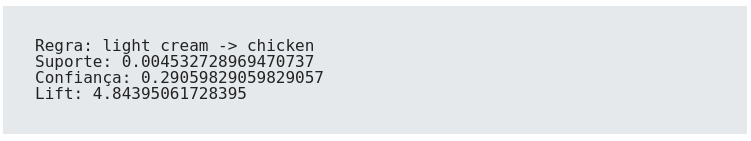
\includegraphics[width=0.7\textwidth]{cap05/apriori1}
	\caption{Primeira regra obtida}
\end{figure}

Entre o "Frango" e o "Creme Light". O valor de suporte é 0,0045 (este número é calculado dividindo o número de transações que contêm o primeiro produto dividido pelo número total de transações). A confiança de 0,2905 significa que de todas as transações que contêm "Creme Light", 29,05\% também foi comprado "Frango". \textit{Lift} mostra que o "Creme Light" tem 4,84 vezes mais chances de ser comprado pelos clientes que compram "Frango", em comparação com a probabilidade de venda do "Creme Light".

Para fixarmos vejamos a próxima regra:
\begin{figure}[H]
	\centering
	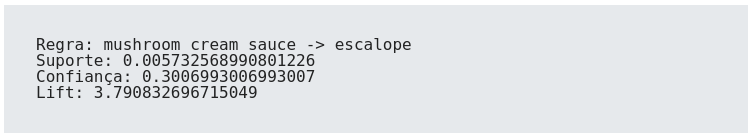
\includegraphics[width=0.7\textwidth]{cap05/apriori2}
	\caption{Segunda regra obtida}
\end{figure}

Entre o "Molho de Creme de Cogumelos" e o "Escalope". O suporte é de 0,0057. A confiança de 0,3006 significa que de todas as transações que contêm o "Molho de Creme de Cogumelos" 30,06\% também contêm "Escalope". \textit{Lift} mostra que o "Escalope" tem 3,79 mais chances de ser comprado pelos clientes que compram o "Molho de Creme de Cogumelos", em comparação com a probabilidade de venda do "Escalope".

Pronto, agora já podemos ler todas as outras 46 regras criadas entre os produtos e aumentar as vendas do nosso negócio.

\section{SVM}\index{Modelos Preditivos}
\textit{Support Vector Machine} é um algorítimo supervisionado capaz de classificar, regredir e também encontrar outliers. Para entendê-lo vamos considerar a seguinte figura:
\begin{figure}[H]
	\centering
	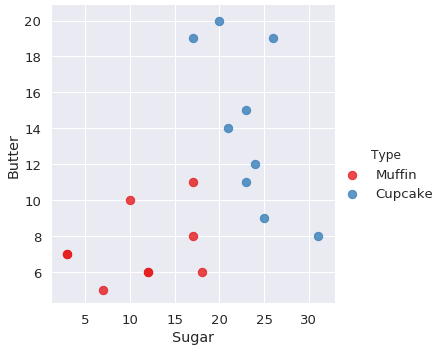
\includegraphics[width=0.6\textwidth]{cap05/svm1}
	\caption{Comparação Muffin e Cupcake}
\end{figure}

Devemos nos perguntar aonde poderíamos colocarmos uma reta que separaria os dois grupos da melhor forma possível? Compreendendo isso matamos esse algorítimo. A nossa base será formada por percentuais com várias receitas de Muffin e Cupcake.

A função que daremos ao algorítimo será de identificar se trata de um ou outro. Vamos começar com a importação das bibliotecas necessárias:
\begin{lstlisting}[]
import pandas as pd
import numpy as np
from sklearn import svm
from sklearn import datasets
from sklearn.metrics import confusion_matrix
import matplotlib.pyplot as plt
import seaborn as sns; sns.set(font_scale=1.2)

%matplotlib inline
\end{lstlisting}

O algorítimo da SVM está na Scikit-Learn, porém precisamos entender que existem 3 classes distintas para se trabalhar com Classificação: \textbf{SVC}, \textbf{NuSVC} e \textbf{LinearSVC}. SVC e NuSVC são métodos semelhantes, mas possuem alguns parâmetros com algumas pequenas diferenças bem como formulações matemáticas. Por outro lado, o LinearSVC é outra implementação do Modelo para o caso de um kernel linear. Trabalharemos aqui com a SVC ou \textit{C-Support Vector Classification}.

Próximo trabalho é baixar a base \textbf{muffins\_cupcakes.csv} ler:
\begin{lstlisting}[]
recipes = pd.read_csv('bases/muffins_cupcakes.csv')
recipes.head()
\end{lstlisting}

Basicamente essa base contém as proporções dos seguintes ingredientes: Farinha (\textit{Flour}), Leite (\textit{Milk}), Açúcar (\textit{Sugar}), Manteiga (\textit{Butter}), Ovo (\textit{Egg}), Fermento (\textit{Baking Powder}), Essência de Baunilha (\textit{Vanilla}) e Sal (\textit{Salt}). Vamos separar Açúcar e Manteiga para treinar nosso modelo:
\begin{lstlisting}[]
ingrediente = recipes[['Sugar', 'Butter']].values
tipo = np.where(recipes['Type']=='Muffin', 0, 1)
\end{lstlisting}

E como é um modelo supervisionado, precisamos também indicar do que se trata a receita. Treinamos nosso modelo:
\begin{lstlisting}[]
model = svm.SVC(kernel='linear', decision_function_shape=None)
model.fit(ingrediente, tipo)
\end{lstlisting}

Uma vez feito isso, vamos criar dois pontos para definir uma linha (apenas para mostrar) como nossos dados são separados:
\begin{lstlisting}[]
w = model.coef_[0]
a = -w[0] / w[1]
xx = np.linspace(5, 30)
yy = a * xx - (model.intercept_[0]) / w[1]
\end{lstlisting}

Agora basta colocarmos tudo em um gráfico:
\begin{lstlisting}[]
sns.lmplot('Sugar', 'Butter', data=recipes, hue='Type', palette='Set1', fit_reg=False, scatter_kws={"s": 70});
plt.plot(xx, yy, linewidth=2, color='black');
\end{lstlisting}

E obtemos o seguinte resultado:
\begin{figure}[H]
	\centering
	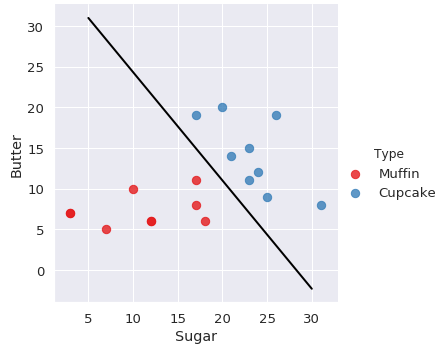
\includegraphics[width=0.6\textwidth]{cap05/svm2}
	\caption{Comparação Muffin e Cupcake}
\end{figure}

Mas como essa linha é encontrada? Isso é feito com base em "margens". Criamos mais 2 linhas para entendermos o processo:
\begin{lstlisting}[]
b = model.support_vectors_[0]
yy_down = a * xx + (b[1] - a * b[0])
b = model.support_vectors_[-1]
yy_up = a * xx + (b[1] - a * b[0])
\end{lstlisting}

E ao colocar novamente tudo em um gráfico:
\begin{lstlisting}[]
sns.lmplot('Sugar', 'Butter', data=recipes, hue='Type', palette='Set1', fit_reg=False, scatter_kws={"s": 70})
plt.plot(xx, yy, linewidth=2, color='black')
plt.plot(xx, yy_down, 'k--')
plt.plot(xx, yy_up, 'k--')
plt.scatter(model.support_vectors_[:, 0], model.support_vectors_[:, 1], s=80, facecolors='none');
\end{lstlisting}

E obtemos o seguinte resultado:
\begin{figure}[H]
	\centering
	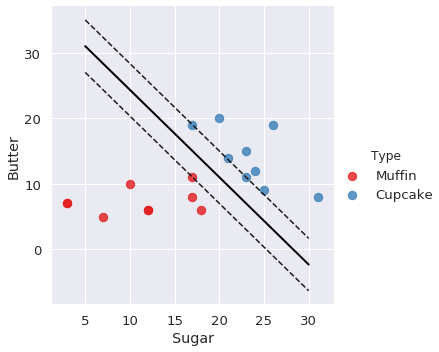
\includegraphics[width=0.6\textwidth]{cap05/svm3}
	\caption{Comparação Muffin e Cupcake}
\end{figure}

E é exatamente a partir da melhor "margem" que a linha é criada. O mais interessante que esse é um algorítimo de previsão, então vamos criar um pequeno método:
\begin{lstlisting}[]
def muffin_ou_cupcake(sugar, butter):
  if (model.predict([[sugar, butter]])) == 0:
    print('Isto é uma receita de Muffin')
  else:
    print('Isto é uma receita de Cupcake')
\end{lstlisting}

E podemos fazer algumas verificações:
\begin{lstlisting}[]
muffin_ou_cupcake(20, 10)
\end{lstlisting}

E isso nos diz que provavelmente trata-se de um Muffin!

\subsection{Retorno a Íris}\index{Modelos Preditivos}

Vamos retornar as nossas flores para entendermos mais algumas coisas sobre esse modelo:
\begin{lstlisting}[]
iris = datasets.load_iris()
df = pd.DataFrame(data=np.c_[iris['data'], iris['target']], columns=iris['feature_names'] + ['Species'])
df.head()
\end{lstlisting}

Separamos nossos dados em duas massas:
\begin{lstlisting}[]
X = df.iloc[:, :4]
y = df.Species
\end{lstlisting}

Lembramos que as 4 primeiras informações são as variáveis explanatórias e a última define qual a espécie. Vamos então treinar nosso algorítimo:
\begin{lstlisting}[]
clf = svm.SVC()
clf.fit(X, y)
\end{lstlisting}

E verificamos o resultado sobre a Matriz de Confusão:
\begin{figure}[H]
	\centering
	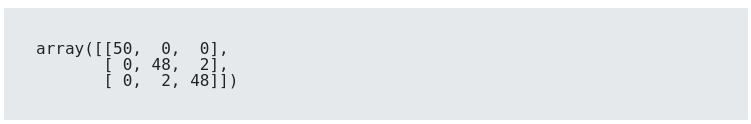
\includegraphics[width=0.7\textwidth]{cap05/svm4}
	\caption{Resultado da Matriz de Confusão}
\end{figure}

Ou seja, 4 espécies foram classificadas erradas. Podemos melhorar esse resultado com a adição de alguns parâmetros:
\begin{itemize}[nolistsep]
	\item \textbf{C}: parâmetro de regularização
	\item \textbf{kernel}: que pode ter um dos seguintes valores linear, poly, rbf, sigmoid, precomputed.
\end{itemize}
	
Após alguns testes chegamos na seguinte configuração para treino do nosso modelo:
\begin{lstlisting}[]
clf = svm.SVC(C=1, kernel='linear')
clf.fit(X, y)
\end{lstlisting}

E agora o resultado da Matriz de Confusão é:
\begin{figure}[H]
	\centering
	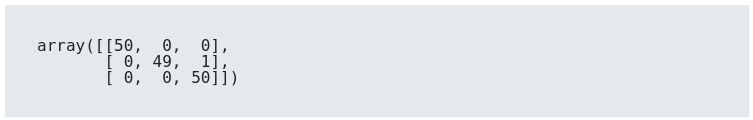
\includegraphics[width=0.7\textwidth]{cap05/svm5}
	\caption{Resultado Final da Matriz de Confusão}
\end{figure}

E temos uma excelente resposta desse modelo.

\section{Regressão Logística}\index{Modelos Preditivos}
Já vimos sobre a \textbf{Regressão Linear} e sobre sua capacidade "Preditiva" sobre valores contínuos, pensemos em Preços de Imóveis, Preço de Ações ou mesmo Previsão do Tempo. Porém em se tratando de variáveis categóricas, do tipo, isso é um email ou não? Essa pessoa pode ou não querer um seguro? Em qual partido votará? Precisamos ter uma outra forma de previsão. Esse é o objetivo da Regressão Logística, que é utilizada como uma das técnicas de classificação (o modelo anterior também era um classificador).

Os problemas de classificação se envolvem em dois tipos: Binários - o cliente quer ou não um seguro? e Multiclasse - em qual partido votará? Vamos começar com o tipo Binário e futuramente veremos o outro. Iniciamos com a importação das nossas bibliotecas:
\begin{lstlisting}[]
import pandas as pd
import matplotlib.pyplot as plt
from sklearn.linear_model import LogisticRegression
from scipy.special import expit

%matplotlib inline
\end{lstlisting}

Se compararmos com o Modelo de Regressão Linear temos a mesma classe Linear Model da Scikit-Learn porém com o método LogisticRegression para realizar nosso trabalho. E o método expit que utilizaremos para traçar a "sigmóide". Agora baixamos a base \textbf{insurance\_data.csv} e a lemos:
\begin{lstlisting}[]
df = pd.read_csv('bases/insurance_data.csv')
df.head()
\end{lstlisting}

Os dados para o "Seguro de Vida" que utilizamos, contém duas variáveis: a idade e se possui (valor 1) ou não (valor 0) um seguro. Próximo passo é treinar nosso modelo com esses dados:
\begin{lstlisting}[]
reg = LogisticRegression()
reg.fit(df[['age']], df.bought_insurance)
\end{lstlisting}

E realizamos nossas previsões:
\begin{lstlisting}[]
reg.predict([[43], [25]])
\end{lstlisting}

Alguém com idade de 43 ou 25 anos desejará adquirir um seguro? E teremos como resposta: array([1, 0]), indicando sim para 43 anos e não para 25.

\subsection{Função Sigmóide}\index{Modelos Preditivos}
Como a mágica acontece? Através de uma função chamada sigmóide, também chamada "função de achatamento". Matematicamente falando, essa função é assim: $f(x) = \frac{1}{1 + e^{-x}}$. Podemos implementá-la da seguinte forma:
\begin{lstlisting}[]
from scipy.optimize import curve_fit
import numpy as np

def funcao_sigmoide(x, x0, k):
  y = 1.0 / (1 + np.exp(-np.dot(k, x-x0)))
  return y

popt, pconv = curve_fit(funcao_sigmoide, df['age'], df.bought_insurance)
sigmoide = funcao_sigmoide(df['age'], *popt)
\end{lstlisting}

Porém a função expit (da biblioteca SciPy) já realiza toda essa implementação, sendo assim, tudo isso pode ser substituído por:
\begin{lstlisting}[]
sigmoide = expit(df['age'] * reg.coef_[0][0] + reg.intercept_[0])
\end{lstlisting}

O que facilita bastante nossa codificação, plotamos os dados:
\begin{lstlisting}[]
plt.plot(df['age'], sigmoide)
plt.scatter(df['age'], df.bought_insurance, c=df.bought_insurance, cmap='rainbow', edgecolors='b')
plt.show()
\end{lstlisting}

E o resultado final será esse:
\begin{figure}[H]
	\centering
	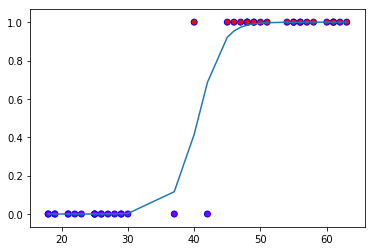
\includegraphics[width=0.5\textwidth]{cap05/rl2}
	\caption{Curva da Sigmóide para nossos dados}
\end{figure}

\subsection{Com mais Variáveis}\index{Modelos Preditivos}
A base de dados que usaremos é bem interessante, mostra os dados de empréstimos concedidos a estudantes, baixar o arquivo \textbf{emprestimo.csv}. Devemos prever se um potencial aquisitor do empréstimo será ou não um bom pagador.

Iniciamos com a importação das bibliotecas necessárias:
\begin{lstlisting}[]
import pandas as pd
from sklearn.linear_model import LogisticRegression
from sklearn.model_selection import train_test_split
from sklearn.preprocessing import LabelEncoder
from sklearn.metrics import accuracy_score
from matplotlib import pyplot as plt

%matplotlib inline
\end{lstlisting}

Para em seguida ler os dados:
\begin{lstlisting}[]
data = pd.read_csv('bases/emprestimo.csv')
data.show()
\end{lstlisting}

E temos os seguintes dados a nossa disposição com um total de 614 linhas:
\begin{figure}[H]
	\centering
	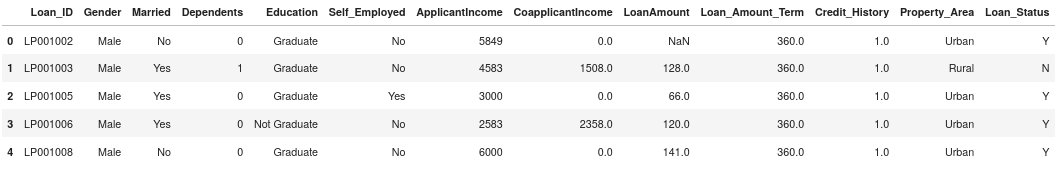
\includegraphics[width=1.0\textwidth]{cap05/rl3}
	\caption{Dados de Empréstimo}
\end{figure}

A variável explanatória chama-se "Loan\_Status" o que indica se o estudante é ou não um bom pagador. Primeiro problema que temos é transformar a variável explanatória em 0 ou 1, pois o modelo que estamos espera esse tipo de variável:
\begin{lstlisting}[]
encode = LabelEncoder()
data.Loan_Status = encode.fit_transform(data.Loan_Status)
\end{lstlisting}

Na segunda parte desse tratamento eliminamos as variáveis que não contribuem para o resultado final (neste caso somente a Loan\_ID) e qualquer linha que possua o valor nulo:
\begin{lstlisting}[]
# Retirar o campo Loan_ID
data = data.drop(columns=['Loan_ID'], axis=1)
# Limpeza dos valores nulos
data.dropna(how='any',inplace=True)
\end{lstlisting}

E isso nos faz perder 22\% dos dados e temos agora 480 linhas. Lembre-se sempre que o corte dos nulos deve ser realizado de forma cirúrgica e não com um machado\footnote{o programa que utilizo para realizar esse tratamento é o \textit{OpenRefine} mas como não é o tema aqui sugiro que veja uma apostila que publiquei sobre este software}. Nosso próximo passo é separar nossa amostra em treino e teste:
\begin{lstlisting}[]
X_train, X_test, y_train, y_test = train_test_split(data.drop(columns=['Loan_Status'],axis=1), data['Loan_Status'], test_size = .2)
\end{lstlisting}

Normalmente deixamos 20\% para teste e verificação da acurácia do modelo esse número pode ser aumentado ou diminuído conforme seus dados, não existe uma regra definida. Modelos de regressão trabalham com variáveis numéricas, então vamos transformar nossas descritivas:
\begin{lstlisting}[]
X_train = pd.get_dummies(X_train)
X_test = pd.get_dummies(X_test)
\end{lstlisting}

O método \textit{get\_dummies} transformará todas as variáveis em dados lógicos. Por exemplo para gênero temos duas: Gender\_Female e Gender\_Male. Assim e realizado sucessivamente para todas as outras. Executamos o modelo e verificamos a acurácia:
\begin{lstlisting}[]
clf = LogisticRegression(max_iter=200)
clf.fit(X_train, y_train)
print('Acurácia:', clf.score(X_test, y_test))
\end{lstlisting}

E verificamos 75\% de precisão, um outro meio de obtermos a acurácia seria pelo método acuracy\_score():
\begin{lstlisting}[]
y_pred = clf.predict(X_test)
print('Acurácia:', accuracy_score(y_test, y_pred))
\end{lstlisting}

Como trabalhamos com um modelo de Regressão Logística não existe maneira de colocar todas as variáveis (até existe, mas vira uma bela confusão) em um único gráfico. Assim analisamos separadamente:

\begin{lstlisting}[]
plt.rcParams['figure.figsize'] = (10,8)
df = pd.DataFrame({'ApplicantIncome': X_test['ApplicantIncome'], 'Correto': y_test, 'Predito': y_pred})
df = df.sort_values(by=['ApplicantIncome'])
plt.scatter(df['ApplicantIncome'], df['Correto'], color='red', marker='+')
plt.plot(df['ApplicantIncome'], df['Predito'], color='blue', linewidth=2)
plt.show()
\end{lstlisting}

E obtemos o seguinte gráfico:
\begin{figure}[H]
	\centering
	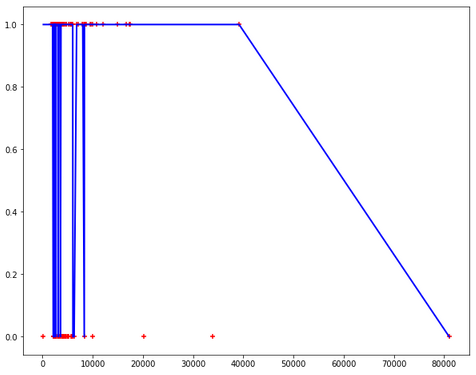
\includegraphics[width=0.45\textwidth]{cap05/rl4}
	\caption{Gráfico sobre pagadores}
\end{figure}

E observamos que até o valor de \$ 10.000 existe uma "indecisão" sobre se o estudante é ou não um bom pagador. Acima disso torna-se um bom pagador (com 2 exceções). Ou seja, precisamos das outras variáveis para ver como o modelo realmente se comportam:
\begin{lstlisting}[]
plt.rcParams['figure.figsize'] = (25,20)
for i, e in enumerate(X_test.columns):
  df = pd.DataFrame({e: X_test[e], 'Correto': y_test, 'Predito': y_pred})
  df = df.sort_values(by=[e])
  ax = plt.subplot(5, 4, i+1)
  ax.scatter(df[e], df['Correto'], color='red', marker='+')
  ax.plot(df[e], df['Predito'], color='blue', linewidth=2)
  ax.set_title(str(e))
plt.show()
\end{lstlisting}

Usamos um laço for para percorrer toda a lista de variáveis e obtemos o seguinte resultado:
\begin{figure}[H]
	\centering
	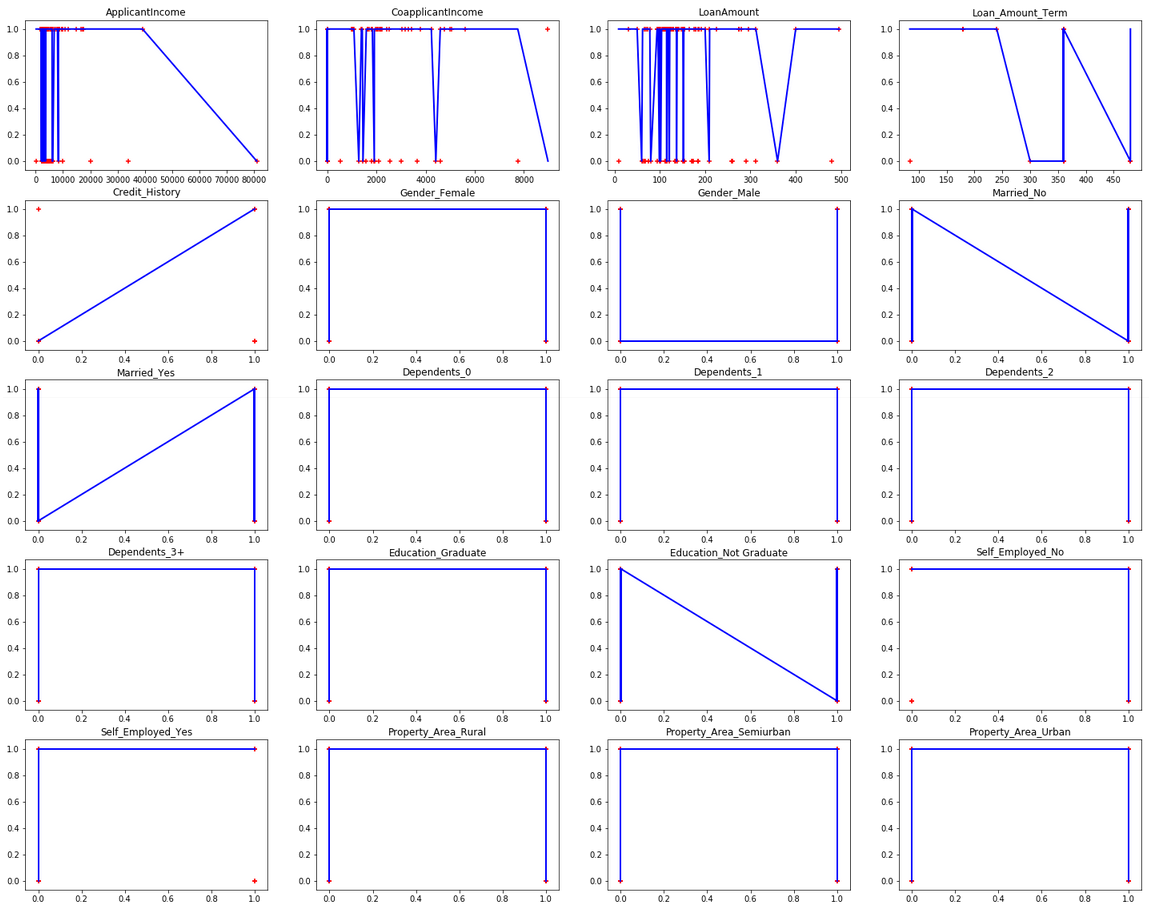
\includegraphics[width=0.8\textwidth]{cap05/rl5}
	\caption{Gráficos aplicado a todas as variáveis}
\end{figure}

E podemos verificar como todas se comportam. Não espere encontrar sigmóides perfeitas em seus dados, isso é uma exceção e não um comportamento padrão.
\clearpage
 